\chapter{Анализ исходных данных}

\section{Загрузка файла с данными}

Загрузку файла с данными можно выполнить разными способами, но мы воспользуемся тем, который не требует установки дополнительных пакетов:

\begin{minted}[fontsize=\small]{r}
data <- read.table(file      = "data.csv",
                   header    = TRUE,
                   sep       = ";",
                   row.names = 1)
\end{minted}

У загруженных данных есть один недостаток -- неудобные длинные имена для столбцов. Однако, это можно исправить с помощью следующей команды:

\begin{minted}[fontsize=\small]{r}
names(data) <- c("Группа",
                 "Пол",
                 "Возраст",
                 "Стаж",
                 "Процент успеха",
                 "Количество ошибок",
                 "Оценка заказчика",
                 "Удовлетворенность заказчика",
                 "Качество документации")
\end{minted}

Также, согласно варианту, есть две подгруппы программистов: со стажем больше 4 лет и меньше 4 лет. Назовем первую подгруппу <<juniors>>, а вторую <<seniors>>. Проведем выборку программистов для каждой подгруппы и занесем их в соответствующие переменные:

\begin{minted}[fontsize=\small]{r}
juniors <- subset(data, data$Группа == 1)
seniors <- subset(data, data$Группа == 2)
\end{minted}

Эти группы выделены для удобства использования в дальнейшем. Вместо того, чтобы каждый раз задавать подмножество всей выборки, будем обращаться к созданным переменным.


\section{Расчет основных статистических характеристик}

К основным можно отнести такие статистические характеристики как:
\begin{itemize}
	\item среднее арифметическое;
	\item медиана;
	\item стандартное отклонение;
	\item дисперсия;
	\item абсолютное отклонение медианы;
	\item сумма;
	\item минимальное значение;
	\item максимальное значение;
	\item мода;
	\item первая квартиль;
	\item третья квартиль.
\end{itemize}

Расчет этих параметров по столбцам может сообщить важную и интересную информацию, но это не всегда так. Например, найдя сумму по столбцу <<Группа>> сложно будет получить из нее сколько-нибудь значимую информацию.

Вообще, выборка содержит следующие поля, которые стоит подвергнуть статистическому анализу:

\begin{itemize}
	\item пол (количественная);
	\item возраст (количественная);
	\item стаж (количественная);
	\item процент успеха (количественная);
	\item количество ошибок (количественная);
	\item оценка заказчика (количественная);
	\item удовлетворенность заказчика (качественная);
	\item качество документации (количественная).
\end{itemize}

Для простоты вычисления основных статистических показателей напишем функцию, которая принимает параметр из выборки и считает показатели для него, а затем возвращает вектор значений, где каждый столбец подписан нужным критерием.

\begin{minted}[fontsize=\small]{r}
get_stat <- function(x) {
	x_mean   <- mean(x)
	x_median <- median(x)
	x_sd     <- sd(x)
	x_var    <- var(x)
	x_mad    <- mad(x)
	x_sum    <- sum(x)
	x_diff   <- diff(x)
	x_min    <- min(x)
	x_max    <- max(x)
	x_q1     <- quantile(x, c(0.25, 0.75))
	x_uniq   <- unique(x)
	x_mode   <- x_uniq[which.max(tabulate(match(x, x_uniq)))]
	return(c("Среднее"                       = x_mean,
	         "Медиана"                       = x_median,
	         "Стандартное отклонение"        = x_sd,
	         "Дисперсия"                     = x_var,
	         "Абсолютное отклонение медианы" = x_mad,
	         "Сумма"                         = x_sum,
	         "Минимальное значение"          = x_min,
	         "Максимальное значение"         = x_max,
	         "Квартили"                      = x_q1,
	         "Мода"                          = x_mode))
}
\end{minted}

\newpage

\subsection{Характеристики первой группы}
К первой группе программистов (juniors) относятся те, чей стаж в компании меньше четырех лет. Размер выборки --- 100 человек.

\begin{table}[H]
	\centering
	\caption{Характеристики пола первой группы}
	\begin{tabular}{|l|c|}
		\hline
		\multicolumn{1}{|c|}{\textbf{Показатель}} & \textbf{Значение}\\ \hline
		Среднее арифметическое        & 1.4       \\ \hline
		Медиана                       & 1         \\ \hline
		Стандартное отклонение        & 0.492366  \\ \hline
		Дисперсия                      & 0.2424242 \\ \hline
		Абсолютное отклонение медианы & 0         \\ \hline
		Сумма                         & 140       \\ \hline
		Минимальное значение          & 1         \\ \hline
		Максимальное значение         & 2         \\ \hline
		Мода & 1 \\ \hline
		Первая квартиль & 1 \\ \hline
		Третья квартиль & 2 \\ \hline
	\end{tabular}
\end{table}


\begin{table}[H]
	\centering
	\caption{Характеристики возраста первой группы}
	\begin{tabular}{|l|c|}
		\hline
		\multicolumn{1}{|c|}{\textbf{Показатель}} & \textbf{Значение}\\ \hline
		Среднее арифметическое        & 28.7     \\ \hline
		Медиана                       & 29       \\ \hline
		Стандартное отклонение        & 1.666667 \\ \hline
		Дисперсия                      & 2.777778 \\ \hline
		Абсолютное отклонение медианы & 1.4826   \\ \hline
		Сумма                         & 2870     \\ \hline
		Минимальное значение          & 24       \\ \hline
		Максимальное значение         & 32       \\ \hline
		Мода & 29 \\  \hline
		Первая квартиль & 28 \\ \hline
		Третья квартиль & 30 \\ \hline
	\end{tabular}
\end{table}


\begin{table}[H]
	\centering
	\caption{Характеристики стажа первой группы}
	\begin{tabular}{|l|c|}
		\hline
		\multicolumn{1}{|c|}{\textbf{Показатель}} & \textbf{Значение}\\ \hline
		Среднее арифметическое        & 2.531     \\ \hline
		Медиана                       & 2.5       \\ \hline
		Стандартное отклонение        & 0.4970001 \\ \hline
		Дисперсия                      & 0.2470091 \\ \hline
		Абсолютное отклонение медианы & 0.59304   \\ \hline
		Сумма                         & 253.1     \\ \hline
		Минимальное значение          & 1.5       \\ \hline
		Максимальное значение         & 3.7       \\ \hline
		Мода & 2.1 \\ \hline
		Первая квартиль & 2.1 \\ \hline
		Третья квартиль & 2.9 \\ \hline
	\end{tabular}
\end{table}


\begin{table}[H]
	\centering
	\caption{Характеристики процента успеха первой группы}
	\begin{tabular}{|l|c|}
		\hline
		\multicolumn{1}{|c|}{\textbf{Показатель}} & \textbf{Значение}\\ \hline
		Среднее арифметическое        & 88.22    \\ \hline
		Медиана                       & 83       \\ \hline
		Стандартное отклонение        & 5.748219 \\ \hline
		Дисперсия                      & 33.04202 \\ \hline
		Абсолютное отклонение медианы & 5.9304   \\ \hline
		Сумма                         & 8222     \\ \hline
		Минимальное значение          & 68       \\ \hline
		Максимальное значение         & 99       \\ \hline
		Мода & 83 \\ \hline
		Первая квартиль & 78 \\ \hline
		Третья квартиль & 83 \\ \hline
	\end{tabular}
\end{table}


\begin{table}[H]
	\centering
	\caption{Характеристики количества ошибок первой группы}
	\begin{tabular}{|l|c|}
		\hline
		\multicolumn{1}{|c|}{\textbf{Показатель}} & \textbf{Значение}\\ \hline
		Среднее арифметическое        & 16.86    \\ \hline
		Медиана                       & 16       \\ \hline
		Стандартное отклонение        & 4.355468 \\ \hline
		Дисперсия                      & 18.9701  \\ \hline
		Абсолютное отклонение медианы & 4.4478   \\ \hline
		Сумма                         & 1686     \\ \hline
		Минимальное значение          & 7        \\ \hline
		Максимальное значение         & 27       \\ \hline
		Мода & 15 \\ \hline
		Первая квартиль & 14 \\ \hline
		Третья квартиль & 20 \\ \hline
	\end{tabular}
\end{table}


\begin{table}[H]
	\centering
	\caption{Характеристики оценки заказчика первой группы}
	\begin{tabular}{|l|c|}
		\hline
		\multicolumn{1}{|c|}{\textbf{Показатель}} & \textbf{Значение}\\ \hline
		Среднее арифметическое        & 70.47    \\ \hline
		Медиана                       & 71       \\ \hline
		Стандартное отклонение        & 8.586406 \\ \hline
		Дисперсия                      & 73.72636 \\ \hline
		Абсолютное отклонение медианы & 10.3782  \\ \hline
		Сумма                         & 7047     \\ \hline
		Минимальное значение          & 53       \\ \hline
		Максимальное значение         & 95       \\ \hline
		Мода & 71 \\ \hline
		Первая квартиль & 64 \\ \hline
		Третья квартиль & 77 \\ \hline
	\end{tabular}
\end{table}


\begin{table}[H]
	\centering
	\caption{Характеристики качества документации первой группы}
	\begin{tabular}{|l|c|}
		\hline
		\multicolumn{1}{|c|}{\textbf{Показатель}} & \textbf{Значение}\\ \hline
		Среднее арифметическое        & 2.47      \\ \hline
		Медиана                       & 2         \\ \hline
		Стандартное отклонение        & 0.9369519 \\ \hline
		Дисперсия                      & 0.8778788 \\ \hline
		Абсолютное отклонение медианы & 1.4826    \\ \hline
		Сумма                         & 247       \\ \hline
		Минимальное значение          & 1         \\ \hline
		Максимальное значение         & 4         \\ \hline
		Мода & 2 \\ \hline
		Первая квартиль & 2 \\ \hline
		Третья квартиль & 3 \\ \hline
	\end{tabular}
\end{table}






\subsection{Характеристики второй группы}
Ко второй группе программистов (seniors) относятся те, чей стаж в компании больше четырех лет. Размер выборки --- 100 человек.

\begin{table}[H]
	\centering
	\caption{Характеристики пола второй группы}
	\begin{tabular}{|l|c|}
		\hline
		\multicolumn{1}{|c|}{\textbf{Показатель}} & \textbf{Значение}\\ \hline
		Среднее арифметическое        & 1.45 \\ \hline
		Медиана                       & 1    \\ \hline
		Стандартное отклонение        & 0.5  \\ \hline
		Дисперсия                      & 0.25 \\ \hline
		Абсолютное отклонение медианы & 0    \\ \hline
		Сумма                         & 145  \\ \hline
		Минимальное значение          & 1    \\ \hline
		Максимальное значение         & 2    \\ \hline
		Мода & 1 \\ \hline
		Первая квартиль & 1 \\ \hline
		Третья квартиль & 2 \\ \hline
	\end{tabular}
\end{table}


\begin{table}[H]
	\centering
	\caption{Характеристики возраста второй группы}
	\begin{tabular}{|l|c|}
		\hline
		\multicolumn{1}{|c|}{\textbf{Показатель}} & \textbf{Значение}\\ \hline
		Среднее арифметическое        & 32.46    \\ \hline
		Медиана                       & 32       \\ \hline
		Стандартное отклонение        & 2.19006  \\ \hline
		Дисперсия                      & 4.796364 \\ \hline
		Абсолютное отклонение медианы & 1.4826   \\ \hline
		Сумма                         & 3246     \\ \hline
		Минимальное значение          & 26       \\ \hline
		Максимальное значение         & 37       \\ \hline
		Мода & 32 \\ \hline
		Первая квартиль & 31 \\ \hline
		Третья квартиль & 34 \\ \hline
	\end{tabular}
\end{table}


\begin{table}[H]
	\centering
	\caption{Характеристики стажа второй группы}
	\begin{tabular}{|l|c|}
		\hline
		\multicolumn{1}{|c|}{\textbf{Показатель}} & \textbf{Значение}\\ \hline
		Среднее арифметическое        & 6.377     \\ \hline
		Медиана                       & 6.35      \\ \hline
		Стандартное отклонение        & 0.7226292 \\ \hline
		Дисперсия                      & 0.5221929 \\ \hline
		Абсолютное отклонение медианы & 0.66717   \\ \hline
		Сумма                         & 637.7     \\ \hline
		Минимальное значение          & 4.9       \\ \hline
		Максимальное значение         & 8.5       \\ \hline
		Мода & 6.6 \\ \hline
		Первая квартиль & 5.8 \\ \hline
		Третья квартиль & 6.8 \\ \hline
	\end{tabular}
\end{table}


\begin{table}[H]
	\centering
	\caption{Характеристики процента успеха второй группы}
	\begin{tabular}{|l|c|}
		\hline
		\multicolumn{1}{|c|}{\textbf{Показатель}} & \textbf{Значение}\\ \hline
		Среднее арифметическое        & 88.66    \\ \hline
		Медиана                       & 82       \\ \hline
		Стандартное отклонение        & 4.31867  \\ \hline
		Дисперсия                      & 18.65091 \\ \hline
		Абсолютное отклонение медианы & 4.4478   \\ \hline
		Сумма                         & 8266     \\ \hline
		Минимальное значение          & 72       \\ \hline
		Максимальное значение         & 93       \\ \hline
		Мода & 81 \\ \hline
		Первая квартиль & 80 \\ \hline
		Третья квартиль & 86 \\ \hline
	\end{tabular}
\end{table}


\begin{table}[H]
	\centering
	\caption{Характеристики количества ошибок второй группы}
	\begin{tabular}{|l|c|}
		\hline
		\multicolumn{1}{|c|}{\textbf{Показатель}} & \textbf{Значение}\\ \hline
		Среднее арифметическое        & 13.48    \\ \hline
		Медиана                       & 14       \\ \hline
		Стандартное отклонение        & 3.817768 \\ \hline
		Дисперсия                      & 14.57535 \\ \hline
		Абсолютное отклонение медианы & 2.9652   \\ \hline
		Сумма                         & 1348     \\ \hline
		Минимальное значение          & 3        \\ \hline
		Максимальное значение         & 26       \\ \hline
		Мода & 14 \\ \hline
		Первая квартиль & 11 \\ \hline
		Третья квартиль & 16 \\ \hline
	\end{tabular}
\end{table}


\begin{table}[H]
	\centering
	\caption{Характеристики оценки заказчика второй группы}
	\begin{tabular}{|l|c|}
		\hline
		\multicolumn{1}{|c|}{\textbf{Показатель}} & \textbf{Значение}\\ \hline
		Среднее арифметическое        & 74.48    \\ \hline
		Медиана                       & 75       \\ \hline
		Стандартное отклонение        & 8.372007 \\ \hline
		Дисперсия                      & 70.09051 \\ \hline
		Абсолютное отклонение медианы & 7.413    \\ \hline
		Сумма                         & 7448     \\ \hline
		Минимальное значение          & 57       \\ \hline
		Максимальное значение         & 99       \\ \hline
		Мода & 79 \\ \hline
		Первая квартиль & 69.75 \\ \hline
		Третья квартиль & 79 \\ \hline
	\end{tabular}
\end{table}


\begin{table}[H]
	\centering
	\caption{Характеристики качества документации второй группы}
	\begin{tabular}{|l|c|}
		\hline
		\multicolumn{1}{|c|}{\textbf{Показатель}} & \textbf{Значение}\\ \hline
		Среднее арифметическое        & 2.49      \\ \hline
		Медиана                       & 3         \\ \hline
		Стандартное отклонение        & 0.9480975 \\ \hline
		Дисперсия                      & 0.8988889 \\ \hline
		Абсолютное отклонение медианы & 1.4826    \\ \hline
		Сумма                         & 249       \\ \hline
		Минимальное значение          & 1         \\ \hline
		Максимальное значение         & 4         \\ \hline
		Мода & 3 \\ \hline
		Первая квартиль & 2 \\ \hline
		Третья квартиль & 3 \\ \hline
	\end{tabular}
\end{table}







\subsection{Характеристики всей выборки}
Общая группа программистов состоит из 200 человек и не разделяется по выработанному стажу.

\begin{table}[H]
	\centering
	\caption{Характеристики пола общей группы}
	\begin{tabular}{|l|c|}
		\hline
		\multicolumn{1}{|c|}{\textbf{Показатель}} & \textbf{Значение}\\ \hline
		Среднее арифметическое        & 1.425     \\ \hline
		Медиана                       & 1         \\ \hline
		Стандартное отклонение        & 0.4955835 \\ \hline
		Дисперсия                      & 0.245603  \\ \hline
		Абсолютное отклонение медианы & 0         \\ \hline
		Сумма                         & 285       \\ \hline
		Минимальное значение          & 1         \\ \hline
		Максимальное значение         & 2         \\ \hline
		Мода & 1 \\ \hline
		Первая квартиль & 1 \\ \hline
		Третья квартиль & 2 \\ \hline
	\end{tabular}
\end{table}


\begin{table}[H]
	\centering
	\caption{Характеристики возраста общей группы}
	\begin{tabular}{|l|c|}
		\hline
		\multicolumn{1}{|c|}{\textbf{Показатель}} & \textbf{Значение}\\ \hline
		Среднее арифметическое        & 30.58    \\ \hline
		Медиана                       & 30       \\ \hline
		Стандартное отклонение        & 2.705587 \\ \hline
		Дисперсия                      & 7.320201 \\ \hline
		Абсолютное отклонение медианы & 2.9652   \\ \hline
		Сумма                         & 6116     \\ \hline
		Минимальное значение          & 24       \\ \hline
		Максимальное значение         & 37       \\ \hline
		Мода & 30 \\ \hline
		Первая квартиль & 29 \\ \hline
		Третья квартиль & 32 \\ \hline
	\end{tabular}
\end{table}


\begin{table}[H]
	\centering
	\caption{Характеристики стажа общей группы}
	\begin{tabular}{|l|c|}
		\hline
		\multicolumn{1}{|c|}{\textbf{Показатель}} & \textbf{Значение}\\ \hline
		Среднее арифметическое        & 4.454    \\ \hline
		Медиана                       & 4.3      \\ \hline
		Стандартное отклонение        & 2.024643 \\ \hline
		Дисперсия                      & 4.09918  \\ \hline
		Абсолютное отклонение медианы & 2.81694  \\ \hline
		Сумма                         & 890.8    \\ \hline
		Минимальное значение          & 1.5      \\ \hline
		Максимальное значение         & 8.5      \\ \hline
		Мода & 2.1 \\ \hline
		Первая квартиль & 2.5 \\ \hline
		Третья квартиль & 6.325 \\ \hline
	\end{tabular}
\end{table}


\begin{table}[H]
	\centering
	\caption{Характеристики процента успеха общей группы}
	\begin{tabular}{|l|c|}
		\hline
		\multicolumn{1}{|c|}{\textbf{Показатель}} & \textbf{Значение}\\ \hline
		Среднее арифметическое        & 82.44    \\ \hline
		Медиана                       & 83       \\ \hline
		Стандартное отклонение        & 5.075946 \\ \hline
		Дисперсия                      & 25.76523 \\ \hline
		Абсолютное отклонение медианы & 4.4478   \\ \hline
		Сумма                         & 16488    \\ \hline
		Минимальное значение          & 68       \\ \hline
		Максимальное значение         & 99       \\ \hline
		Мода & 81 \\ \hline
		Первая квартиль & 79 \\ \hline
		Третья квартиль & 86 \\ \hline
	\end{tabular}
\end{table}


\begin{table}[H]
	\centering
	\caption{Характеристики количества ошибок общей группы}
	\begin{tabular}{|l|c|}
		\hline
		\multicolumn{1}{|c|}{\textbf{Показатель}} & \textbf{Значение}\\ \hline
		Среднее арифметическое        & 15.17    \\ \hline
		Медиана                       & 15       \\ \hline
		Стандартное отклонение        & 4.422544 \\ \hline
		Дисперсия                      & 19.55889 \\ \hline
		Абсолютное отклонение медианы & 4.4478   \\ \hline
		Сумма                         & 3034     \\ \hline
		Минимальное значение          & 3        \\ \hline
		Максимальное значение         & 27       \\ \hline
		Мода & 15 \\ \hline
		Первая квартиль & 12 \\ \hline
		Третья квартиль & 18 \\ \hline
	\end{tabular}
\end{table}


\begin{table}[H]
	\centering
	\caption{Характеристики оценки заказчика общей группы}
	\begin{tabular}{|l|c|}
		\hline
		\multicolumn{1}{|c|}{\textbf{Показатель}} & \textbf{Значение}\\ \hline
		Среднее арифметическое        & 72.475   \\ \hline
		Медиана                       & 73       \\ \hline
		Стандартное отклонение        & 8.694096 \\ \hline
		Дисперсия                      & 75.58731 \\ \hline
		Абсолютное отклонение медианы & 8.8956   \\ \hline
		Сумма                         & 14495    \\ \hline
		Минимальное значение          & 53       \\ \hline
		Максимальное значение         & 99       \\ \hline
		Мода & 79 \\ \hline
		Первая квартиль & 66 \\ \hline
		Третья квартиль & 79 \\ \hline
	\end{tabular}
\end{table}


\begin{table}[H]
	\centering
	\caption{Характеристики качества документации общей группы}
	\begin{tabular}{|l|c|}
		\hline
		\multicolumn{1}{|c|}{\textbf{Показатель}} & \textbf{Значение}\\ \hline
		Среднее арифметическое        & 2.48      \\ \hline
		Медиана                       & 3         \\ \hline
		Стандартное отклонение        & 0.9402234 \\ \hline
		Дисперсия                      & 0.8830201 \\ \hline
		Абсолютное отклонение медианы & 1.4826    \\ \hline
		Сумма                         & 496       \\ \hline
		Минимальное значение          & 1         \\ \hline
		Максимальное значение         & 4         \\ \hline
		Мода & 3 \\ \hline
		Первая квартиль & 2 \\ \hline
		Третья квартиль & 3 \\ \hline
	\end{tabular}
\end{table}


\subsection{Характеристики качественных данных}
Не все столбцы в наборе данных являются количественными. Так, например, столбец <<Удовлетворенность заказчика>> относится к качественным данным. Чтобы работать с таким типом данных, необходимо каким-либо образом трансформировать его в количественный.

В нашем случае, можно заметить, что данные в столбце <<Удовлетворенность заказчика>> принимают всего три значения:
\begin{itemize}
	\item низкая;
	\item средняя;
	\item высокая.
\end{itemize}

Трансформация таких данных не вызывает особых трудностей. Их можно отобразить на множество $\{1, 2, 3\}$ соответственно. После этого к ним можно применить точно такие же функции, что и к количественным данным.

Преобразование можно выполнить с помощью следующих команд:
\begin{minted}[fontsize=\small]{r}
index <- data$`Удовлетворенность заказчика` == "низкая"
data[index, "Удовлетворенность заказчика"] <- as.numeric(1)
index <- data$`Удовлетворенность заказчика` == "средняя"
data[index, "Удовлетворенность заказчика"] <- as.numeric(2)
index <- data$`Удовлетворенность заказчика` == "высокая"
data[index, "Удовлетворенность заказчика"] <- as.numeric(3)
data[, "Удовлетворенность заказчика"] <- 
    as.numeric(data[, "Удовлетворенность заказчика"])

\end{minted}

\begin{table}[H]
	\centering
	\caption{Характеристики удовлетворенности заказчика первой группы}
	\begin{tabular}{|l|c|}
		\hline
		\multicolumn{1}{|c|}{\textbf{Показатель}} & \textbf{Значение}\\ \hline
		Среднее арифметическое        & 2.03      \\ \hline
		Медиана                       & 2         \\ \hline
		Стандартное отклонение        & 0.797154  \\ \hline
		Дисперсия                      & 0.6354545 \\ \hline
		Абсолютное отклонение медианы & 1.4826    \\ \hline
		Сумма                         & 203       \\ \hline
		Минимальное значение          & 1         \\ \hline
		Максимальное значение         & 3         \\ \hline
		Мода & 2 \\ \hline
		Первая квартиль & 1 \\ \hline
		Третья квартиль & 3 \\ \hline
	\end{tabular}
\end{table}

\begin{table}[H]
	\centering
	\caption{Характеристики удовлетворенности заказчика второй группы}
	\begin{tabular}{|l|c|}
		\hline
		\multicolumn{1}{|c|}{\textbf{Показатель}} & \textbf{Значение}\\ \hline
		Среднее арифметическое        & 2.31      \\ \hline
		Медиана                       & 2         \\ \hline
		Стандартное отклонение        & 0.747994  \\ \hline
		Дисперсия                      & 0.5594949 \\ \hline
		Абсолютное отклонение медианы & 1.4826    \\ \hline
		Сумма                         & 231       \\ \hline
		Минимальное значение          & 1         \\ \hline
		Максимальное значение         & 3         \\ \hline
		Мода & 3 \\ \hline
		Первая квартиль & 2 \\ \hline
		Третья квартиль & 3 \\ \hline
	\end{tabular}
\end{table}

\begin{table}[H]
	\centering
	\caption{Характеристики удовлетворенности заказчика общей группы}
	\begin{tabular}{|l|c|}
		\hline
		\multicolumn{1}{|c|}{\textbf{Показатель}} & \textbf{Значение}\\ \hline
		Среднее арифметическое        & 2.17      \\ \hline
		Медиана                       & 2         \\ \hline
		Стандартное отклонение        & 0.7836905 \\ \hline
		Дисперсия                      & 0.6141709 \\ \hline
		Абсолютное отклонение медианы & 1.4826    \\ \hline
		Сумма                         & 434       \\ \hline
		Минимальное значение          & 1         \\ \hline
		Максимальное значение         & 3         \\ \hline
		Мода & 3 \\ \hline
		Первая квартиль & 2 \\ \hline
		Третья квартиль & 2 \\ \hline
	\end{tabular}
\end{table}





\subsection{Выводы}
Анализируя полученные результаты можно сделать следующие выводы:

\begin{enumerate}
	\item Во обоих группах гендерное распределение склоняется в сторону мужчин. В группе juniors 60\% мужчин и 40\% женщин, а в группе seniors 55\% мужчин и 45\% женщин. Всего среди программистов представленных в выборке 42.5\% женщин и 57.5\% мужчин.
	
	\item Средний возраст программистов в общем -- 30.58 лет. В группе juniors -- 28.7 лет, а в группе seniors -- 32.46 лет. При этом разброс возрастов для группы seniors лежит на отрезке от 26 до 37 лет. Для группы juniors -- на отрезке от 24 до 32 лет. Суммарно все программисты прожили 6116 лет.
	
	\item В среднем люди проработали в компании 4.454 года. При этом самый последний программист был нанят 1.5 года назад, а самый <<старый>> 8.5 лет назад.Суммарно все программисты посвятили компании 890.8 лет.
	
	\item Группа juniors закрывает успешно 88.22\% задач за год. Самый неэффективный работник по этой метрике закрывает 68\% задач, а самый эффективный -- 99\%. В группе seniors успешно выполняется 88.66\% задач. Диапазон эффективности от 72\% до 93\%. В общем все программисты работают с эффективностью 82.44\%. Процент закрытия задач примерно одинаков, однако важно понимать, что, скорее всего, более опытные разработчики реализуют гараздо более сложные и важные задачи. Также человек с самым низким показателем не обязательно является лентяем. Вполне вероятно, что часть задач, которые он решал потребовали от него гораздо больше времени и сил на решение из-за чего он не смог закрыть остальные.
	
	\item Количество ошибок, которые допускают программисты колеблется от 3 до 27. Всего за год обнаруживается 3034 ошибки. В среднем на каждого программиста приходится по 15.17 ошибки. В группе siniors в среднем обнаруживается 13.48 ошибки. При этом максимальное количество допущенных ошибок 1 программистом равно 26. В группе juniors в среднем допускается 16.86 ошибки в год. При этом минимальное количество ошибок равно 7 против 3 у группы seniors. Все допускают ошибки, но явно видно, что опыт сказывается, и разработчики со стажем допускают меньше ошибок.
	
	\item Заказчик оценивает работу программиста в среднем на 72.475 балла из 100. Самая низкая оценка от заказчика -- 53, а самая высокая 99. В группе juniors средняя оценка составляет 70.47 баллов, а в группе seniors -- 74.48 балла. Из чего может следовать, что группа seniors выполняет свою работу несколько лучше.
	
	\item Заказчик в общем удовлетворен чуть выше среднего.
	
	\item Качество документации в среднем составляет 2.48 балла. Максимальная оценка за документацию равна 4, а минимальная -- 1. Можно сказать, что разработчики не особо стремятся составлять документацию к производимым продуктам.
\end{enumerate}











\section{Графический анализ данных}

\subsection{Графики}

\begin{figure}[H]
	\centering
	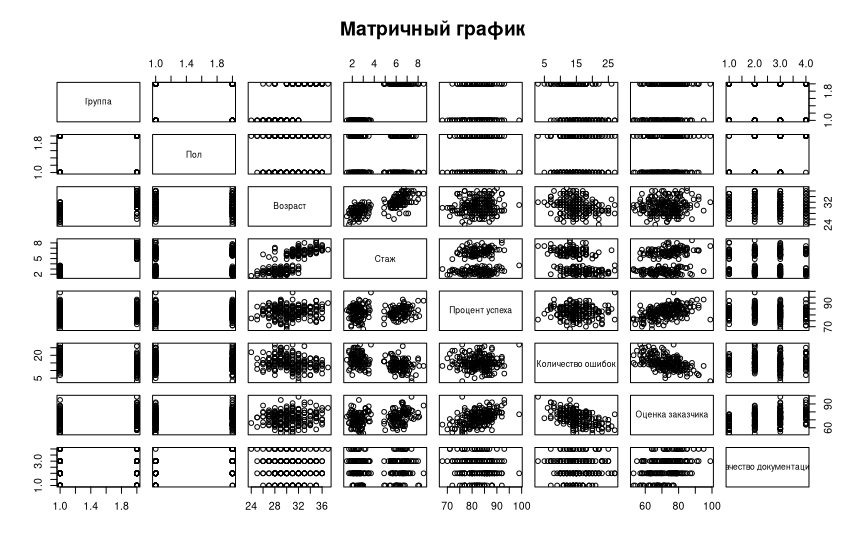
\includegraphics[width=\linewidth]{fig1}
	\caption{Диаграмма рассеяния по двум количественным признакам}
\end{figure}

\begin{figure}[H]
	\centering
	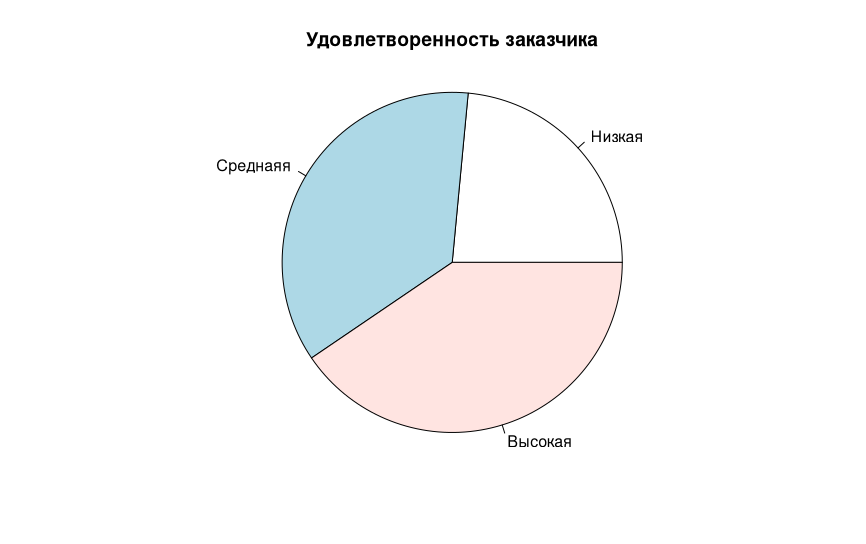
\includegraphics[width=\linewidth]{fig2}
	\caption{Радиальная диаграмма по качественному признаку}
\end{figure}

\begin{figure}[H]
	\centering
	
	\caption{Категориальная радиальная диаграмма по одному из качественных признаков в зависимости от пола и группы}
\end{figure}

\begin{figure}[H]
	\centering
	
	\caption{Категориальная столбиковая диаграмма по одному из количественных признаков в зависимости от пола и группы}
\end{figure}

\begin{figure}[H]
	\centering
	
	\caption{Диаграмму размаха для одного из количественных признаков в зависимости от значений пола или группы}
\end{figure}

\begin{figure}[H]
	\centering
	
	\caption{Гистограммы для всех количественных признаков на одном графике}
\end{figure}

\begin{figure}[H]
	\centering
	
	\caption{Матричный график по всем количественным переменным}
\end{figure}

\subsection{Выводы}














\section{Корреляционный анализ данных}

\subsection{Степень взаимосвязи между качественными переменными}

\subsection{Степень взаимосвязи между количественными переменными}

\subsection{Степень взаимосвязи между двумя количественными переменными}

\subsection{Графическое представление матриц коэффициентов корреляции}